\documentclass[11pt, oneside]{article}      % use "amsart" instead of "article" for AMSLaTeX format
\usepackage[top=1.25in, bottom=1.25in]{geometry}                       % See geometry.pdf to learn the layout options. There are lots.
\geometry{letterpaper}                          % ... or a4paper or a5paper or ... 
%\geometry{landscape}                       % Activate for for rotated page geometry
\usepackage[parfill]{parskip}           % Activate to begin paragraphs with an empty line rather than an indent
\usepackage{graphicx}               % Use pdf, png, jpg, or eps§ with pdflatex; use eps in DVI mode
                                % TeX will automatically convert eps --> pdf in pdflatex        
\usepackage{amssymb}
\usepackage{amsmath}

\newcommand{\word}{\textnormal{word}}
\newcommand{\lemma}{\textnormal{lemma}}

\title{Machine Translation \\ Final Project Interim Report}
\author{Jeremy Silver}
\date{Tues.\ 4/21/15}                          % Activate to display a given date or no date

\begin{document}
\maketitle

The purpose of my project is to explore the body of formal linguistic theory and its potential utility for machine translation.  While great MT successes have been derived from purely statistical methods, the state-of-the-art systems now seem to be gravitating steadily towards the incorporation of higher-level linguistic features, such as syntactic parsing and lexical semantics.  

The holy grail of machine translation is the conversion of text into an ``interlingua,'' or a formal representation of the meaning that allows for inter-translation between languages, as well as the potential for automated inference.  The language of first-order (or higher-order) logic is a strong candidate for this interlingua since it has vast expressive capability, and since the advancement of theorem-proving and model-building software in recent years has opened the door to more sophisticated logical reasoning.

The paradigm I have chosen to experiment with is that of Noam Chomsky's \textit{generative grammar}, in particular the X-bar theory framework that has grown out of Chomsky's original program from the 1960s and 70s.  This is to be contrasted with his more recent \textit{minimalist} program, which uses dependency-based grammars instead of tree-based constituency grammars.  There has been a lot of promising research on dependency structures in MT, perhaps most noteworthy the \textit{Abstract Meaning Representation} project, which seeks to encode a large number of conceptual relations in DAG (directed acyclic graph) structures.  While such a representation may soon become a central locus of future MT research, I have eschewed it for the purposes of my experiments due to its learning curve and its syntactic flexibility (which may ultimately be a strength rather than a weakness).

Crucial to X-bar theory is the notion of \textit{constituency}, which asserts that there are meaningful subunits of language (phrases), bigger than words, but smaller than sentences.  There is a great deal of evidence for this, but one example is the \textit{replacement test}, in which an already-used phrase can be substituted with an anaphoric construction:

\begin{enumerate}
\item Bill had a big brown dog, and Sally had a small white one.
\item Bill had a big brown dog, and Sally had a small one.
\item Bill had a big brown dog, and Sally had one too.
\item Bill had a big brown dog, and Sally did too.
\end{enumerate}

This sequence of examples shows that \textit{dog}, \textit{brown dog}, \textit{big brown dog}, and \textit{had a big brown dog} are all constituents, since they can each be replaced by an anaphor.  Every constituent has a \textit{head}, which is a subconstituent that confers its part of speech to the overall phrase.  The head of a noun phrase is a noun, so that even when modified by numerous adjectives or prepositional phrases, the noun phrase still behaves grammatically like a noun.  This is what allows the entire phrase ``big brown dog'' to be replaced by a single noun ``one'' in example 3.

Two major strengths of the theory are its recursive nature (since we know that language behaves recursively, as in ``I know that you know that I know that you know...'') and its generality.  In fact, X-bar theory can essentially be boiled down to three rules: 

\begin{enumerate}
\item Specifier rule: \quad XP $\rightarrow$ (YP) X$'$
\item Adjunct rule:   \quad  X$'$ $\rightarrow$ (ZP) X$'$
\item Complement rule: \quad X$'$ $\rightarrow$ (WP) X
\end{enumerate}

These are generative diagrams; for example, the specifier rule means that if XP is a phrase of category X, it can be decomposed into an (optional) phrase of category Y, and a head ``X-bar," which is a constituent of category X that is in an intermediate state between an X and an XP.  The distinction between an X, an X$'$, and an XP is simply a convenience of notation; it allows us to distinguish between a lexical item (X), an intermediate projection (X$'$), and a maximal or ``complete'' projection (XP).  Also, the above rules assume the language is ``head-final'', but the order of the decompositions could be switched around depending on the particular language.  The paucity of these generation rules, as well as the fact that they are at most binary-branching, means that X-bar theory can be an effective framework for context-free grammar (CFG) parsing.

To recap, X-bar theory posits that a sentence can be represented as a binary tree in which every subtree is a constituent.  Its category is determined by its head, and binary (or unary) branching occurs based on one of the three rules given above.  To put this methodology into practice, for the experimental component of my project I have implemented a CFG-based parser for a fragment of English that is capable of parsing and sketching diagrams for simple sentences in the X-bar theoretic framework.  See Figure 1 for an X-bar parsing of the canonical sentence, ``Every farmer has a donkey."  One will notice a lot of seemingly extraneous nodes; these are the unary projections that are required for conformity to the theory.  It is also worth noting that we have distinct phrasal categories DP and NP for determiner and noun phrases.  The distinction has to do with quantification, which I hope to touch on in my final report.  Also, TP is a separate category from VP in that the latter is an un-tensed verb phrase, while the former includes tense, aspect, and modality.

\begin{figure}[h] \label{fig_sent1}
\caption{A sentence parsed in X-bar theory}
\centerline{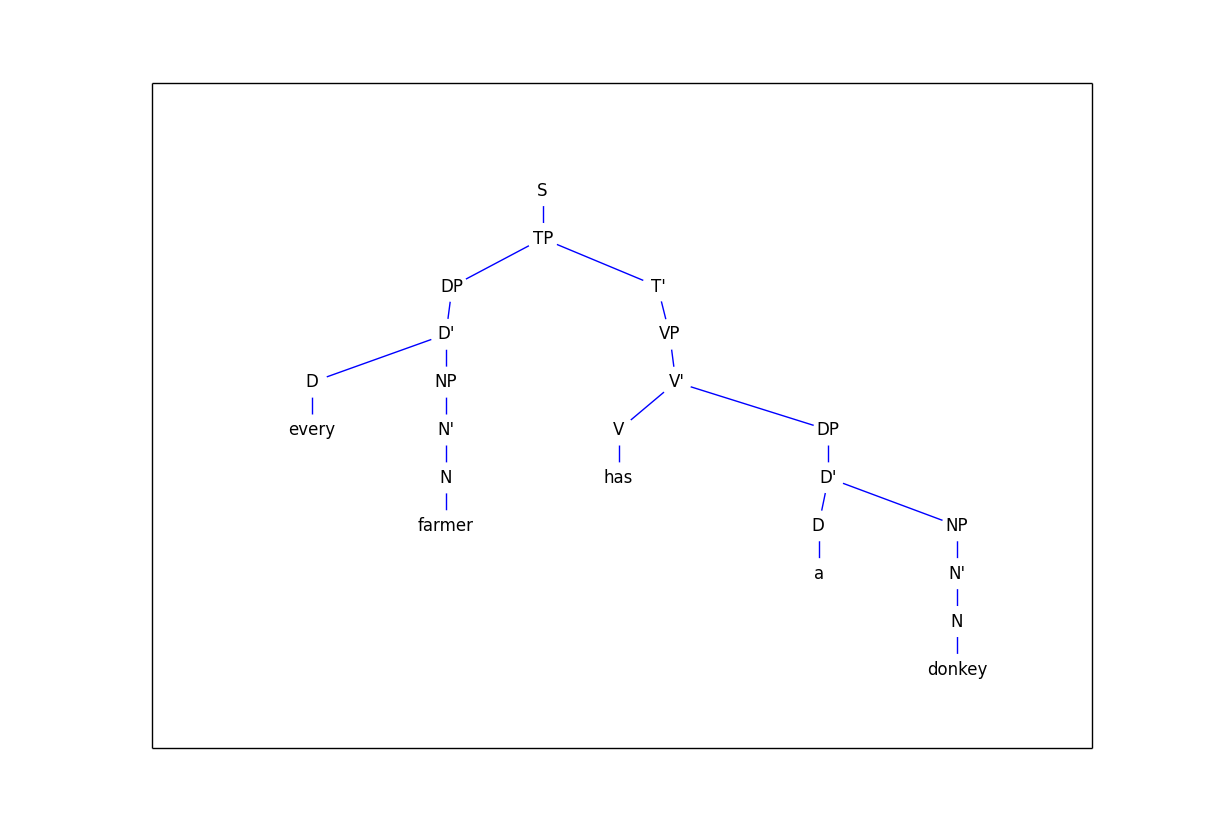
\includegraphics[scale=.6]{sent1.png}}
\end{figure}

Two factors that can significantly complicate things are \textit{ambiguity}, in which there are multiple valid parse trees for a given sentence, and \textit{movement}, in which constituents move to other places in the tree in order to check morphological or semantic features.  For example, in English we have \textit{subject-aux inversion}, leading us to say ``Where did you go?" instead of ``Where you went?''  The hypothesis of Chomskyan grammar is that there is an underlying logical form that gets expressed as a ``deep syntactic structure'', and then a series of transformations is applied before the sentence is actually expressed in its surface form.  To get the underlying deep structure, these transformations will have to be applied in reverse.  This can be a very challenging computational problem, which we will not worry about for the moment.

Once a sentence is syntactically parsed, it can be converted into a logical statement via Frege's principle of \textit{compositionality}.  Starting from the leaf nodes, each of which has a logical representation, each constituent can be assigned a meaning by composing the meanings of its daughter nodes.  The main driver of this composition is \textit{function application}, whereby one node is a function that takes its sister as an argument, and output of the function is the composed meaning.  If this condition is not met, the phrase is \textit{uninterpretable}.  In order to have a well-defined procedure for function application, all meanings must be assigned a \textit{type}.  Following the basic conventions in formal semantic theory, we say that $e$ and $t$ are the basic types, and that if $\sigma$ and $\tau$ are types, then ${<}\sigma, \tau{>}$ is the type of functions from $D_{\sigma}$ to $D_{\tau}$, where $D_{\sigma}$ and $D_{\tau}$ are the domains of objects with types $\sigma$ and $\tau$ respectively.  The set $D_e$ is the set of primitive ``entities,'' or ``things in the universe,'' while $D_t = \{0, 1\}$ is the set of truth values.  Sentences have $t$ as their semantic type, individuals have $e$ as their type, and unary predicates (like intransitive verbs) have ${<}e, t{>}$ as their type.

For a simple example of compositionality via function application, take ``John runs.'' If the meaning of ``John'' is some entity labeled JOHN $\in D_e$, and the meaning of ``runs'' is the characteristic function labeled RUN of some set of entities (the ones that run), i.e.\ an element of $D_{<e, t>}$, then the meaning of ``John runs'' is simply the function RUN applied to the argument JOHN, with a return value of type $t$.  It may seem like we have gained nothing by simply capitalizing the words, but in reality we have created a formal representation of a sentence, where we have simply chosen to leave JOHN and RUN as atomic concepts.  Other words, however, may be semantically reduced.  For example, we could choose to represent the word ``bachelor'' by $\lambda x \, . \, MAN(x) \wedge \neg MARRIED(x).$  In this notation we have introduced a \textit{lambda function}, in this case, a mapping from $x$ to a truth value of 1 if and only if $x$ is a man and $x$ is not married.  

In this style of semantic representation, we are allowed to remain agnostic on what the words \textit{actually} mean, and leave that to the lexicographers and philosophers.  For the purposes of machine translation, a deeper understanding of meaning is not very necessary, since it is only necessary for us to be able to map English words to foreign words, and the logical representation is only an intermediary.

While there is much more to be said on the topic of compositional semantics, I will save that discussion for the final report, and I will now propose a method for ``perfect translation'' of sentences from English to another language using logical form as a medium:

\begin{enumerate}
\item Parse the English sentence into X-bar theory.
\item Apply movement operations in reverse to derive the deep syntactic structure.
\item Interpret the sentence bottom-up, starting from the leaves, using lexical lookups and the compositionality principle.  Terminate if any constituent is uninterpretable.  Annotate the syntax tree at every node with its partial semantic representation.
\item Once the logical form is derived, apply any simplification operations to the syntax tree or logical form, as needed.
\item For each constituent in the English tree, attempt to derive syntax trees in the foreign language for the same constituent using heuristics and reverse lexical lookups (mapping from meanings to words). If a constituent cannot be generated, try to go up one level in the tree and derive that instead. A combination of top-down recursion and bottom-up projection may be needed.
\item When the target logical form has been generated in the foreign language, apply syntactic/morphological transformations to the foreign tree to get the foreign surface form.
\end{enumerate}

Each of these steps can be quite challenging.  Python's Natural Language Toolkit (NLTK) has tools available that can make steps 1-3 fairly straightforward.  It will be my primary goal to get up to this point for a body of example English sentences, ranging in complexity from ``John runs'' to ``Every farmer has a donkey,'' which features the quantifier scope ambiguity that is a persistent challenge to linguists.  Time permitting, I will try to implement at least a proof-of-concept for the remaining steps to derive translations of simple sentences into Japanese, a language I am familiar with that is syntactically quite different from English.

One of the main motivations for attempting a syntax/semantics-driven approach to MT is that it can resolve certain issues involving complicated syntactic structures. For example, passive voice is often mistranslated in standard MT so that the subject and object roles are reversed.  A fully syntax-aware system will not make such a mistake.  Another example is when the two languages use completely different syntactic structures to convey the same meaning.  For example, take the simple sentence, ``John likes Mary."  In Japanese, this would be rendered, ``John wa Mary ga suki desu," which literally means something like, ``For John, Mary is favored."  What was formerly the object of a transitive verb is now the subject of an adjectival predicate.  Google Translate does manage to get this right, but either it is already using the syntactic rule or else it will be incapable of maintaining the proper transformation over long distances.

A final motivation for this type of method is that it is expert-driven rather than data-driven.  Obviously using data has its advantages, but it also has drawbacks.  First, there is usually the requirement of large parallel corpora, which may be unavailable for certain languages.  The large amount of data may be superfluous anyway if the language can be encoded in a handful of simple rules.  Instead of spending many hours on intensive training algorithms, the syntactic model and the lexicon will be designed from the start to incorporate the nuanced insights of human experts.  Also, the logical interlingua will serve as a gateway between any pair of languages, not just a single pair.

Again, it is not my immediate intention to outperform even basic statistical machine translation techniques, but rather to compare and contrast these techniques with a more rule-based approach driven by formal linguistic theory.  In the final report I also plan to discuss ways in which statistical methods would still be pivotal in the rule-based approach, for example, in disambiguating word senses and in incorporating phrases as basic lexical entries.

\begin{thebibliography}{1}

\bibitem{amr} {\em Abstract Meaning Representation (AMR) 1.2 Specification}. amr.isi.edu.

\bibitem{bosBlackburn} Blackburn, Patrick, and Johan Bos.  Computational Semantics.  {\em Theoria}, 18(1), pages 365-387, 2003.

\bibitem {carnie} Carnie, Andrew. {\em Syntax: A Generative Introduction}. Blackwell, 2007.

\bibitem {heim} Heim, Irene, and Angelika Kratzer.  {\em Semantics in Generative Grammar}.  Blackwell, 1998.

\end{thebibliography}

\end{document}  
